\begin{statementbox}
\textbf{C093\quad 共焦椭圆与双曲线公共点的焦半径公式}

\textbf{条件：}左、右焦点分别是 $F_1=(-c,0)$、$F_2=(c,0)$，$c>0$。
椭圆 $E$ 使用小写半轴 $a,b$，双曲线 $H$ 使用大写半轴 $A,B$，
两曲线标准方程分别为
\[
\boxed{E:\ \frac{x^2}{a^2}+\frac{y^2}{b^2}=1},\qquad
\boxed{H:\ \frac{x^2}{A^2}-\frac{y^2}{B^2}=1}.
\]
其中
\[
a>b>0,\quad A>0,\ B>0,\qquad
a^2-b^2=A^2+B^2=c^2,\quad c>0.
\]
因此 $a>c>A>0$。点 $P=(x_P,y_P)$ \emph{同时在 $E$ 和 $H$ 上}。

\begin{center}
% C093: a=4, A=1, c=2; E: x^2/16+y^2/12=1, H: x^2-y^2/3=1
% Intersection P=(2,3); PF1=5, PF2=3; generated as exact coordinate constructions.
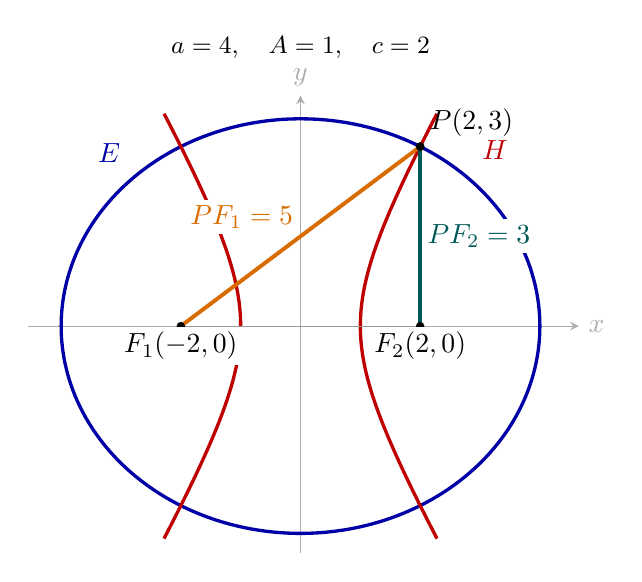
\begin{tikzpicture}[scale=0.76,>=stealth]
 \node[font=\small] at (0,4.65) {$a=4,\quad A=1,\quad c=2$};
 \draw[->,gray!65] (-4.55,0)--(4.65,0) node[right]{$x$};
 \draw[->,gray!65] (0,-3.8)--(0,3.85) node[above]{$y$};
 \draw[blue!65!black,very thick,samples=160,domain=0:360,smooth,variable=\t]
  plot ({4*cos(\t)},{sqrt(12)*sin(\t)});
 \draw[red!75!black,very thick,samples=110,domain=-3.55:3.55,variable=\t]
  plot ({sqrt(1+\t*\t/3)},{\t});
 \draw[red!75!black,very thick,samples=110,domain=-3.55:3.55,variable=\t]
  plot ({-sqrt(1+\t*\t/3)},{\t});
 \coordinate (L) at (-2,0); \coordinate (R) at (2,0); \coordinate (P) at (2,3);
 \draw[orange!85!black,line width=1.4pt] (L)--(P) node[midway,above left,fill=white,inner sep=2pt]{$PF_1=5$};
 \draw[teal!70!black,line width=1.4pt] (R)--(P) node[midway,right,fill=white,inner sep=2pt]{$PF_2=3$};
 \draw[gray!80] (L)--(R);
 \fill (L) circle (2pt) node[below,fill=white,inner sep=2pt]{$F_1(-2,0)$};
 \fill (R) circle (2pt) node[below,fill=white,inner sep=2pt]{$F_2(2,0)$};
 \fill (P) circle (2.1pt) node[above right]{$P(2,3)$};
 \node[blue!65!black] at (-3.2,2.9) {$E$};
 \node[red!75!black] at (3.25,2.95) {$H$};
\end{tikzpicture}

\end{center}

\textbf{主结论（未指定左右支时）：}
\[
\boxed{\{PF_1,PF_2\}=\{a+A,\ a-A\}},\qquad a>c>A>0.
\]
花括号只表示\emph{这两种长度}，尚不指定哪一个属于 $PF_1$。

\textbf{指定左右支后：}
\[
\boxed{\begin{array}{ll}
\text{右支 }x_P>0:& PF_1=a+A,\quad PF_2=a-A,\\[3pt]
\text{左支 }x_P<0:& PF_1=a-A,\quad PF_2=a+A.
\end{array}}
\]
位于同一支上方或下方的两个公共点，到相应焦点的距离相同。

\end{statementbox}
\clearpage
\begin{statementbox}
\textbf{结论续：离心率形式}

\textbf{离心率形式：}令椭圆离心率 $e_1=c/a$、
双曲线离心率 $e_2=c/A$，则 $0<e_1<1<e_2$，
\[
\boxed{\{PF_1,PF_2\}
=\left\{c\left(\frac1{e_1}+\frac1{e_2}\right),\ 
 c\left(\frac1{e_1}-\frac1{e_2}\right)\right\}}.
\]
\textbf{适用信号：}“椭圆、双曲线共焦”并且“求同一个公共点的焦半径”。
\end{statementbox}
